\begin{tikzpicture}
    \node [mybox] (box) {
        \begin{minipage}{0.48\textwidth}
            \begin{tabular}{lp{0.5\textwidth}}
                Binary Cross Entropy $\arg \min_{\theta} =$ & 
                \sloppy
                $
                    - \frac{1}{N} \sum^N 
                            \left[ r_{ui} \log(\tilde{p}_{ui}(\theta)) 
                            + (1 - r_{ui}) \log(\tilde{p}_{ui}(\theta)) \right]
                $
                \\
                Sampling &
                    \begin{itemize}[label={--}, topsep=0cm, parsep=0cm, itemsep=0cm]
                        \item[$\times$] Cannot use ground truth (too many negative samples)
                        \item[$\times$] Cannot use just positive samples (no learning)
                        \item[$\checkmark$] Subsample among + and - interaction with probability $p=0.5$
                    \end{itemize}
                
                \\

                % --- AUTOENCODERS ---
                \textbf{Autoencoder} & \\
                \hline
                Reconstruction Loss & MSE, BCE
                \\
                Steps & 
                \begin{itemize}[label={--}, topsep=0cm, parsep=0cm, itemsep=0cm]
                    \item Sample a user profile $r_u$
                    \item Ecode it $e_u = g_e(r_u)$
                    \item Decode it $\tilde{r}_u = g_d(e_u)$
                    \item Rank the items
                \end{itemize}
                \\
                
                % --- EaseR ---
                \textit{EaseR} & (Item-Based similarity CF model)
                \\
                \hline
                Loss Function $S^* = $ & 
                $
                    \arg \min_{S} 
                    || R - RS ||_F 
                    + \lambda || S ||_F 
                    +  2\vec{\gamma} \odot diag(S)
                $

                $
                    \vec{\gamma} \in \mathbb{R}^{|I|}
                $
                \\
                Constraints & 
                $
                    diag(S) = 0
                $
                \\
                Similarity Matrix & 
                $
                    P = (R^T \cdot R + \lambda I_{|I|})^{-1}
                $
                
                $
                    S^* = I_{|I|} - P \cdot diag( \mathbf{1} 
                            \oslash diag(P))
                $
                \\
                Pros and Cons & 
                \begin{itemize}[label={}, topsep=0cm, parsep=0cm, itemsep=0cm]
                    \item[$\checkmark$] Fast and highly efficient
                    \item[$\checkmark$] Due the Frobenius norm, it tries to compute $R = RS$, thus repoducing the input as output such as an autoencoder.
                    \item[$\times$]  Computing P is memory intensive
                \end{itemize}
                \\
            \end{tabular}
            \begin{tcolorbox}[colback=gray!5, colframe=gray!80!black, title={Autoencoders and Item-Item Similarity Correlation}]
                Given a shallow autoencoder with no hidden layers and embedding size $K$, if $f = I$ and $b_e,b_d = 0$ then:
                \begin{center}
                $
                    e_u = f_e(r_u \cdot W_e + b_e) = r_u \cdot W_e
                $

                $
                    \tilde{r}_u = f_d(e_u \cdot W_d + b_d) = e_u \cdot W_d = r_u \cdot W_e \cdot W_d
                $
                \end{center}

                Since 
                $
                    W_e \in \mathbb{R}^{|I| \times K}, W_d \in \mathbb{R}^{|K| \times |I|}
                $

                We can derive the assymmetric (or symmetric, if encoder and decoder share parameters) similarity matrix $S$ as:
                $
                    S = W_e \cdot W_d
                $
            \end{tcolorbox}
        \end{minipage}
    };


    \node[fancytitle, right=10pt] at (box.north west) {DL for RECSYS};
\end{tikzpicture}


\begin{tikzpicture}
    \node [mybox] (box) {
        \begin{minipage}{0.48\textwidth}
            \begin{tabular}{lp{0.5\textwidth}}
                 % -- denoising %
                 Denoising Autoecoders & \\
                
                 \hline
 
                 Risks &
                 \begin{itemize}[label={}, topsep=0cm, parsep=0cm, itemsep=0cm]
                     \item[$\times$]  The encoder might create a poor embedding for new user profiles
                     \item[$\times$]  The decoder could lack on reconstruct correctly portion of the embedding space
                 \end{itemize}
                 \\
                 Denoising Salt \& Pepper &
                 \begin{itemize}[label={--}, topsep=0cm, parsep=0cm, itemsep=0cm]
                     \item Dropout, remove a number of positive interactions
                     \item Random add a number of positive interactions
                 \end{itemize}
                 \\

                 % --- Variational Autoencoders ---
                 Variational Autoencoders (Mult-VAE) & Encoding a input as a distribution
                 \\
                 \hline
                 Idea & 
                 \begin{itemize}[label={}, topsep=0cm, parsep=0cm, itemsep=0cm]
                     \item Encoder: encode the input as $\vec{\mu}, \vec{\sigma} $ of a Gaussian
                     \item Decoder: sample from the Gaussian and decode it $\vec{e} \tilde N(\vec{\mu}, \vec{\sigma})$
                     \item Learn the probability distribution $P(\theta | z)$.
                     
                 \end{itemize}
                 \\
                 Reparametrization Trick & 
                 $
                     \vec{e} = \vec{\mu} + \vec{\sigma} \odot \vec{\epsilon}
                 $
                 Where
                 $
                    \vec{\epsilon} \sim \mathcal{N}(0, 1)
                 $
                 \\
                 % --- TWO TOWER MODELS ---
                 \textbf{Two Tower Models} & \\
                 \hline
                  

                 &
                 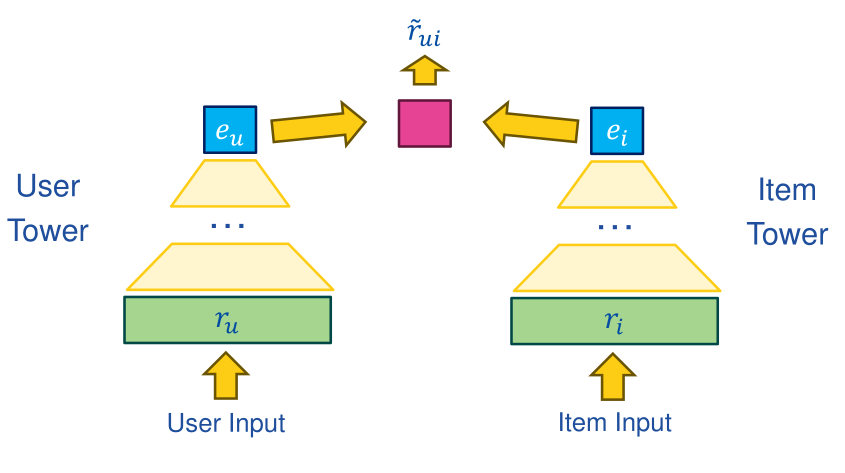
\includegraphics[width=0.35\textwidth]{imgs/090_TwoTowerModel.png}
                 \\
                 Pros and Cons &                 
                 \begin{itemize}[label={--}, topsep=0cm, parsep=0cm, itemsep=0cm]
                     \item[$\checkmark$] Can use any loss function (it does not have to reconstruct the input)
                     \item[$\checkmark$] User and item input can be of different types
                     \item[$\times$] Need to compute several ranking predictions $\tilde{r}_{ui}$
                     \item[$\times$] If the input is a one-hot encoding, it is \textbf{memory based}
                 \end{itemize}
             \end{tabular}
            \begin{tcolorbox}[colback=gray!5, colframe=gray!80!black, title={Two tower models as Matrix Factorization}]
                Consider a two-tower model with no hidden layers, embedding size $K$ and both
                user and item input one-hot encoded $x_u$ , $x_i$. If $f = I$ and $b_u, b_i, I = 0$:
                    
                $\tilde{r}_{ui} =  W_u^U \cdot W_i^I$
                Where
                $
                    W_u^U \in \mathbb{R}^{|U| \times K}, W_i^I \in \mathbb{R}^{|I| \times K}
                $
                Then we have a Matrix Factorization model with $K$ latent factors, $X = W_u^U$ and $Y = W_i^I$
            
            \end{tcolorbox}
                
        \end{minipage}
    };

\node[fancytitle, right=10pt] at (box.north west) {DL for RECSYS - 2};
\end{tikzpicture}